\documentclass[journal]{IEEEtran}


\usepackage{graphicx}
\usepackage{algorithm}
\usepackage{algorithmic}
\usepackage{booktabs}
\usepackage{textcomp}
\usepackage{makecell}
\usepackage{cite}
\usepackage{url}
\usepackage{nomencl}
\usepackage{color}
\makenomenclature


\begin{document}

\newcommand{\tabincell}[2]{\begin{tabular}{@{}#1@{}}#2\end{tabular}}

\title{Improved Rule Installation for Real-time Query Service in Software-Defined Internet of Vehicles}

\author{\authorblockN{Xin Wang, Cheng Wang, Junqi Zhang,~\IEEEmembership{Senior Member,~IEEE,} Mengchu Zhou,~\IEEEmembership{Fellow,~IEEE,} and Changjun Jiang}
\thanks{Xin Wang, Cheng Wang, Junqi Zhang, and Changjun Jiang are with the Department of Computer Science and Engineering, Tongji University, and with the Key Laboratory of Embedded System and Service Computing, Ministry of Education, China. (E-mail: 13xinwang@tongji.edu.cn, cwang@tongji.edu.cn, cjjiang@tongji.edu.cn.)}
\thanks{Mengchu Zhou is with the Department of Electrical and Computer Engineering, New Jersey Institute of Technology, Newark, NJ 07102 USA. (E-mail: mengchu.zhou@njit.edu)}
}

\maketitle


\begin{abstract}
Internet of Vehicles (IoV) has recently gained considerable attentions from both industry and research communities due to the development of communication technology and smart city. However, a proprietary and closed way of operating hardware in network equipment slows down the progress of new service deployment and extension in IoV. Moreover, the tightly coupled control and data planes in traditional networks significantly increase the complexity and cost of network management. By proposing a novel architecture, called Software-Defined Internet of Vehicles (SDIV), we adopt a software-defined network (SDN) architecture to address these problems by leveraging its separation of the control plane from the data one and a uniform way to configure heterogeneous switches. However, the characteristics of IoV introduce some great challenges in rule installation due to the limited size of flow tables at OpenFlow-enabled switches that are the main component of SDN. It is necessary to build compact flow tables for the scalability of IoV. Accordingly, we develop a novel rule installation mechanism to reduce the number of rules for real-time query services in SDIV. Specifically, we separate the wired data plane from wireless one and use multicast addresses in the latter. Furthermore, we introduce a destination-driven model in \textcolor{blue}{the wired data plane} to reduce the number of rules at switches. Experiments with a real data trace show that the developed approach significantly reduces the number of rules without degrading the performance of data transmissions for  real-time query services in IoV.
\end{abstract}

\begin{IEEEkeywords}
Internet of Vehicles (IoV), Software Defined Network (SDN), real-time query service.
\end{IEEEkeywords}

%\IEEEpeerreviewmaketitle

\nomenclature[01]{SDN}{Software-Defined Network}
\nomenclature[02]{IoV}{Internet of Vehicles}
\nomenclature[03]{SDIV}{Software-Defined Internet of Vehicles}
\nomenclature[04]{AP}{Access Point}
\nomenclature[05]{V}{Vehicle}
\nomenclature[06]{TCAM}{Ternary Content-Addressable Memory}
\nomenclature[07]{T}{Timeout for rules at switches}
\nomenclature[08]{D(n, d)}{Euclidean distance between n and d}
\nomenclature[09]{$F_i$}{Data flow i}
\nomenclature[10]{(S, D)}{Packet with the source address S and the destination address D}

\printnomenclature

\section{Introduction}
Internet of Vehicles (IoV) is attracting considerable attention from both academia and industry. The vigorous development of communication technology and smart city makes various services possible in IoV, which significantly improves the quality and safety of human driving. Research and industry communities are carrying out several projects~\cite{CVIS, makino2005smartway} for the development of IoV. For example, EU's CVIS~\cite{CVIS} is committed to the development of the technologies needed to allow cars to communicate with each other and with the nearby roadside infrastructure. Smartway~\cite{makino2005smartway} focuses on integrating all intelligent transportation system functions to a uniform platform and provisioning services by two-way communications.

Though there is a promising future in IoV, the proprietary and closed way of operating devices in networks slows down the deployment and extension of new services in IoV. Network devices such as switches and routers are developed by different manufacturers. Their changes require substantial manual configuration by trained operators, which makes network management expensive and error-prone. The lack of an open and unified interface for flexible and dynamically customizable networks makes it difficult to deploy and extend new services in large-scale IoV. A new network architecture is expected for the development of IoV.

There are several projects for a new network architecture and next-generation Internet. Named Data Networking~\cite{NDN} aims to develop a new Internet architecture that concentrates on getting `what' services rather than `where' to get services. MobilityFirst \cite{MobilityFirst} supports seamless and smooth mobility. It takes the mobility of nodes as a common case rather than a special case in traditional networks. NEBULA \cite{NEBULA} develops a new network architecture based on cloud computing and data centers. Software-Defined Network (SDN) provides a unified interface to configure network equipment and separates a control plane from a data one. A unified interface of configuring network equipment makes a large-scale customizable network possible, and accelerates new service deployment in IoV.

We adopt SDN to support IoV for its open and unified interface, and propose Software-Defined Internet of Vehicles (SDIV), a new architecture for the development of IoV. SDIV has several advantages in supporting IoV besides the open and unified interface: (1) it essentially has high scalability by separating a data plane from a control one, (2) it achieves desired network manageability by using a logically centralized controller, and (3) its controller is able to choose the best path for data transmission and plays as a coordinator for roadside electronic devices according to the current network state. However, IoV characteristics introduce challenges in rule (match and corresponding action) installation due to the limited size of flow tables in its OpenFlow switches. It is thus necessary to build compact flow tables for scalability of IoV.

In this work, we consider real-time query services, that are typical in IoV, to show the design details for improved rule installation in SDIV. Real-time query services provide drivers the real-time road and other information and drivers decide which way to go according to such information. Road information coming from the surveillance cameras (or other kind of roadside electronic devices) is transmitted to every vehicle with demanding. In this scenario, the specific issues are: (1) the mobility of vehicles increases the number of rules since it needs to establish new connections between vehicles and surveillance cameras, and (2) when a vehicle is connecting to multiple cameras, it is not efficient to install rules for every path since it has the same destination. Fig. \ref{fig1} illustrates the issues of rule installation in IoV. If the controller simply installs rules upon the request of drivers, the table size at switches may become the performance bottleneck of a real-time query service in IoV and even fail the service.

\begin{figure} [t]
\begin{center}
\begin{tabular}{cc}
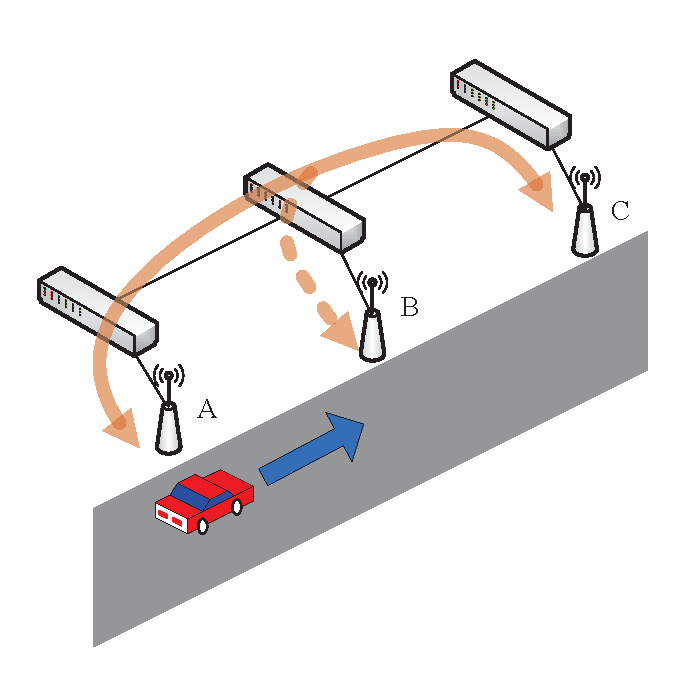
\includegraphics[width=0.48\columnwidth]{fig-1-a-28.eps}&
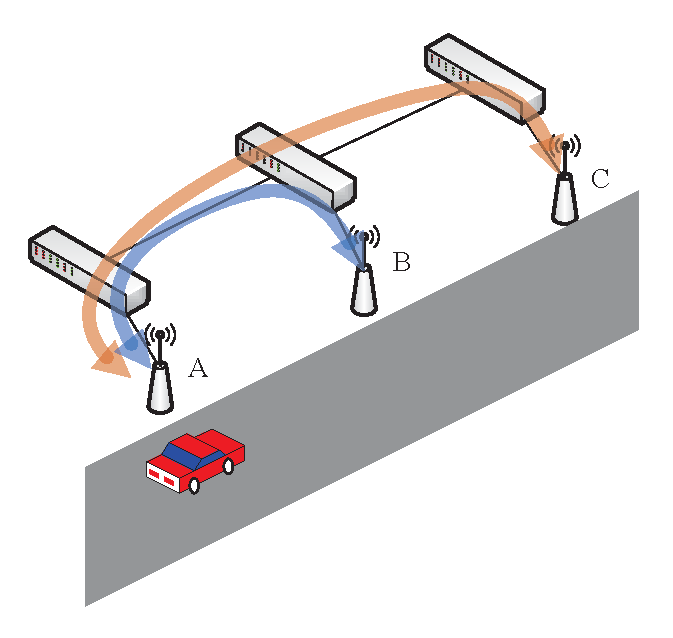
\includegraphics[width=0.48\columnwidth]{fig-1-b-28.eps} \\
(a) & (b)
\end{tabular}
\caption{(a): When a vehicle moves to another place (from $A$ to $B$), it needs to establish a new connection. The dash line represents the connection which is not established yet; (b): When a vehicle \textcolor{blue}{is} connecting to multiple cameras simultaneously, it needs to build a path for each connection which is not efficient since all paths have the same destination (i.e., all data flow's destination is $A$).} \label{fig1}
  \end{center}
  \vspace{-0.3in}
\end{figure}

To address the rule installation and table size growth problems for real-time query services, we develop several techniques by leveraging the centralized and fine granularity of data flow control in SDN for improved rule installation: (1) To reduce the number of requests sent by vehicles, we use multicast addresses instead of general destination address as the last address when vehicles receive data from cameras; (2) To keep uninterrupted connection between vehicles and roadside electronic devices, we install rules in switches in advance based on the conditions of vehicles; and (3) To decrease the number of rules and maintain the correctness of data transmission, we modify the headers when packets come to branching nodes.

In this paper, we first describe the SDIV architecture. We then analyze the problem of flow table size growth in OpenFlow-supported switches. We design and develop an optimization approach to reduce the number of rules in switches. We validate the feasibility of improved rule installation by considering four situations in a real-time query service and analyze the details of data transmission in each case. Finally we use Floodlight~\cite{Floodlight} as a controller and Mininet~\cite{mininet} as a testbed to evaluate the performance of our improved rule installation  method with a real data trace. Experimental results show that when using improved rule installation, the flow table in switches is more compact than simply installing rules without compromising the performance of data communication for real-time query services.

The rest of the paper is organized as follows. In Section~\ref{Related Work}, we review related works. In Section~\ref{Architecture}, we introduce the SDIV architecture. In Section~\ref{Rule Optimization}, we discuss the improved rule installation issues and the proposed solution. We conduct extensive experiments and report results in Section \ref{Evaluation}.  We conclude the paper with future work in Section~\ref{Conclusion}.


\section{Related Work} \label{Related Work}

Most applications and services in IoV, e.g., road security, fleet management, navigation, billing, and multimedia, rely on data transfers between vehicles and roadside infrastructure (V2I) and among vehicles (V2V) \cite{du2015information}.
Several researches \cite{ott2005disconnection, balasubramanian2008interactive} have demonstrated the feasibility of providing connectivity via road-side APs and the ubiquity of WiFi.

The studies \cite{joshi2011vehicular, xu2011utilizing} deal with the efficient communication between APs and vehicles. For routing and data forwarding, \cite{sahu2015bang, zhang2014geomob, zhu2013zoom, nzouonta2009vanet} study the routing protocol and fast forwarding. Routing in IoV in different categories is well reviewed in \cite{cheng2015its}. To manage vehicular networks, a centralized policy framework is introduced and called Virtuoso in \cite{hare2012policy}. It manages spectrum resources while ensuring users to have suitable access to meet their communication needs. In \cite{abadi2015traffic}, traffic flow prediction for traffic forecasting and congestion management is made. The work \cite{wu2013improving} estimates the attitude of a vehicle for low-cost inertial navigation system/GPS. Ahn et al. \cite{ahn2012risa} present the Road Information Sharing Architecture (RISA), representing the first distributed approach to road condition detection and dissemination for vehicular networks. \textcolor{blue}{Calafate et al. \cite{calafate2012efficient} study reliable data delivery through broadcasting by computing the optimal packet size and determining the best Forward Error Correction (FEC) scheme.}

To establish a new architecture in vehicular networks, Grassi et al. \cite{grassi2014vanet} apply Named Data Networking to networking vehicles and enable networking among all computing devices independent of whether they are connected through wired infrastructure, ad hoc, or intermittent Delay Tolerant Network. Yap et al. \cite{yap2010blueprint} present an OpenFlow \cite{mckeown2008openflow} wireless network to achieve a free travel between any wireless infrastructures by separating the network service from the underlying physical infrastructure.

Software-defined network (SDN) is applied to improve network management in \cite{kim2013improving}. A distribution framework is proposed for decomposing large switch tables into small ones to handle limited-size switch tables \cite{kanizo2013palette}, which reduces the flow table size. Voellmy et al. \cite{voellmy2013maple} introduce Maple to discover reusable forwarding decisions and reduce the number of rules by a trace tree structure that records the access to a specific packet.

From the above discussions, we can find that though there are many approaches for IoV development as well as various applications of the SDN concept, there is no or little work of the new service deployment and centralized management in IoV. Thus, we provide an SDIV architecture to do so.



%Mobile social network consists of  mobile users and stationary Access Points (APs).
%APs are deployed in the mobile social network originally, not being as supplementary devices for capacity improvement.
%We model this \emph{hybrid underlying network with APs support} as a \emph{dynamic graph} which can be defined as a time sequence of network graph, denoted by $\mathcal{G} =\{G_{0}, G_{1},...,G_{t},...\}$, where $G_{t}=(V_{t},E_{t})$ represents a time dependent network snapshot recorded at time $t$; $V_{t}$ denotes the set of nodes, including the set of mobile users and the set of stationary APs; $E_{t}=\{(u,v)|u,v\in V_{t}\}$ denotes the edge set. %In terms of the entire network,
%Both node and edge sets change over time.


%\emph{Remark 1}: To cope with the invalidation of Bluetooth devices in those traces, we have $w_{uv}^{t_{p}}=w_{vu}^{t_{p}}$, by assigning the larger value to the other.


%\emph{Remark 2}: Our \emph{weighted} aggregation method avoids the imperfection of the simple growing and sliding time window methods which avoid a social graph   loosing heterogeneity and degenerating to a random graph over time \cite{hossmann2010know}.


\section{Network Architecture: Software-Defined IOV} \label{Architecture}

In this section, we propose an SDIV architecture and discuss its utility through a real-time query service in IoV. Before introducing it, we describe the basic SDN model and its main features.

\subsection{Software Defined Networks (SDN)}\label{SDN}

The principal endeavors of SDN aim to separate the control plane from the data one and centralize a network's intelligence and state to a single device. SDN consists of two parts: (1) switches process flows' packets based on actions of flow entries (i.e. rules) in their flow tables, and (2) the controller generally runs on a remote commodity server and communicates over a secure connection with the switches by using a southbound interface. 

\textcolor{blue}{
\textbf{Controller}: A logical centralized controller connects to all the switches directly or indirectly in the network. It can have a global view (e.g. topology) of the whole network by collecting the state of switches. The controller uses a southbound interface to config the switch for adding or deleting rules.}

\textcolor{blue}{
\textbf{Southbound Interface}: The southbound interface is used by the controller to communicate with the switch. By this interface, the controller can query the state of switches (e.g. bandwidth of links) and also set rules to forward packets. OpenFlow, a protocol maintained by Open Networking Foundation~\cite{ONF}, is viewed as a promising implementation of such an interaction. In this work, we use OpenFlow as the southbound interface between the controller and switches.}

\textcolor{blue}{
\textbf{Rule}: A rule is an entry in the switch's flow table. It consists of match fields, a counter, and a set of actions. When a packet matches a rule's match fields, it applies the corresponding actions and updates the counter. The actions include: (1) Forwarding the packet to particular ports; (2) Dropping the packet; (3) Forwarding the packet to the controller; and (4) Modifying the value of the packet header.}


\subsection{Software-Defined IoV (SDIV)} \label{SDIV}

Our proposed SDIV network has a three-tier architecture. From bottom to top, it has physical, control and application layers, as illustrated in Fig. ~\ref{fig2}.

\subsubsection{Physical Layer}

Physical layer includes vehicles, access points (APs), roadside electronic devices, switches, and servers (different from an SDN controller). Vehicles act as mobile nodes and communicate with the server through road-side APs. When sensors in a vehicle collect conditions of the vehicle, e.g. speed, direction and location, the data should be transmitted to the server as soon as possible. Vehicles receive responses from the server through nearby APs. Note that we assume that the number of road-side APs is sufficient to cover every road. Road-side APs are static WiFi APs reachable from \textcolor{blue}{the road that offers} the capability of data transmission to vehicles. Roadside electronic devices like surveillance cameras gather road conditions and also send data to servers or vehicles. Switches connect APs, surveillance cameras and servers. Servers here provide information service to vehicles, such as road conditions, based on the requests from vehicles and data collected from roadside electronic devices. One vehicle can connect to multiple servers at the same time.

\subsubsection{Control Layer}

In the control layer, the controller connecting to every switch (including APs) acts as a mediator between upper layer applications and underlayer network through SDN. By using OpenFlow, it is able to control all data flows in IoV. Also when the network state changes, the switches (including APs) notify it. In SDIV, they act as a connector among vehicles, servers and other roadside electronic devices by forwarding data flows based on rules which are installed by the controller. Then the controller can convert the strategy of application, e.g., the path selection or access control, into the OpenFlow rules in particular switches, since it has an up-to-date, global view of the network topology and traffic flows. The global network view makes the controller available to provide a customized network state to applications, which is not \textcolor{blue}{possible} in the traditional network. By this means, different applications have different views which benefit both applications and network. The former can have a much simpler view of the network than the detailed, but unnecessary view of the whole network, which can simplify their tasks, e.g., traffic scheduling. For the later, privacy and security benefit from the customized network state which guarantees the former to access their needed data only instead of all data.

\subsubsection{Application Layer}

The strategy of each application is defined in the application layer. Applications provide services for vehicles in IoV, such as a real-time query service, location service and road information service. Each application gets the customized network state from the control layer and makes decisions according to its strategy. The strategy here instructs how to provide services to vehicles. A real-time query service example is to provide drivers the real-time conditions of roads. The network topology is required to compute the path for improving performance, which we will discuss later in Section~\ref{Rule Optimization}.

\begin{figure} [t]
\begin{center}
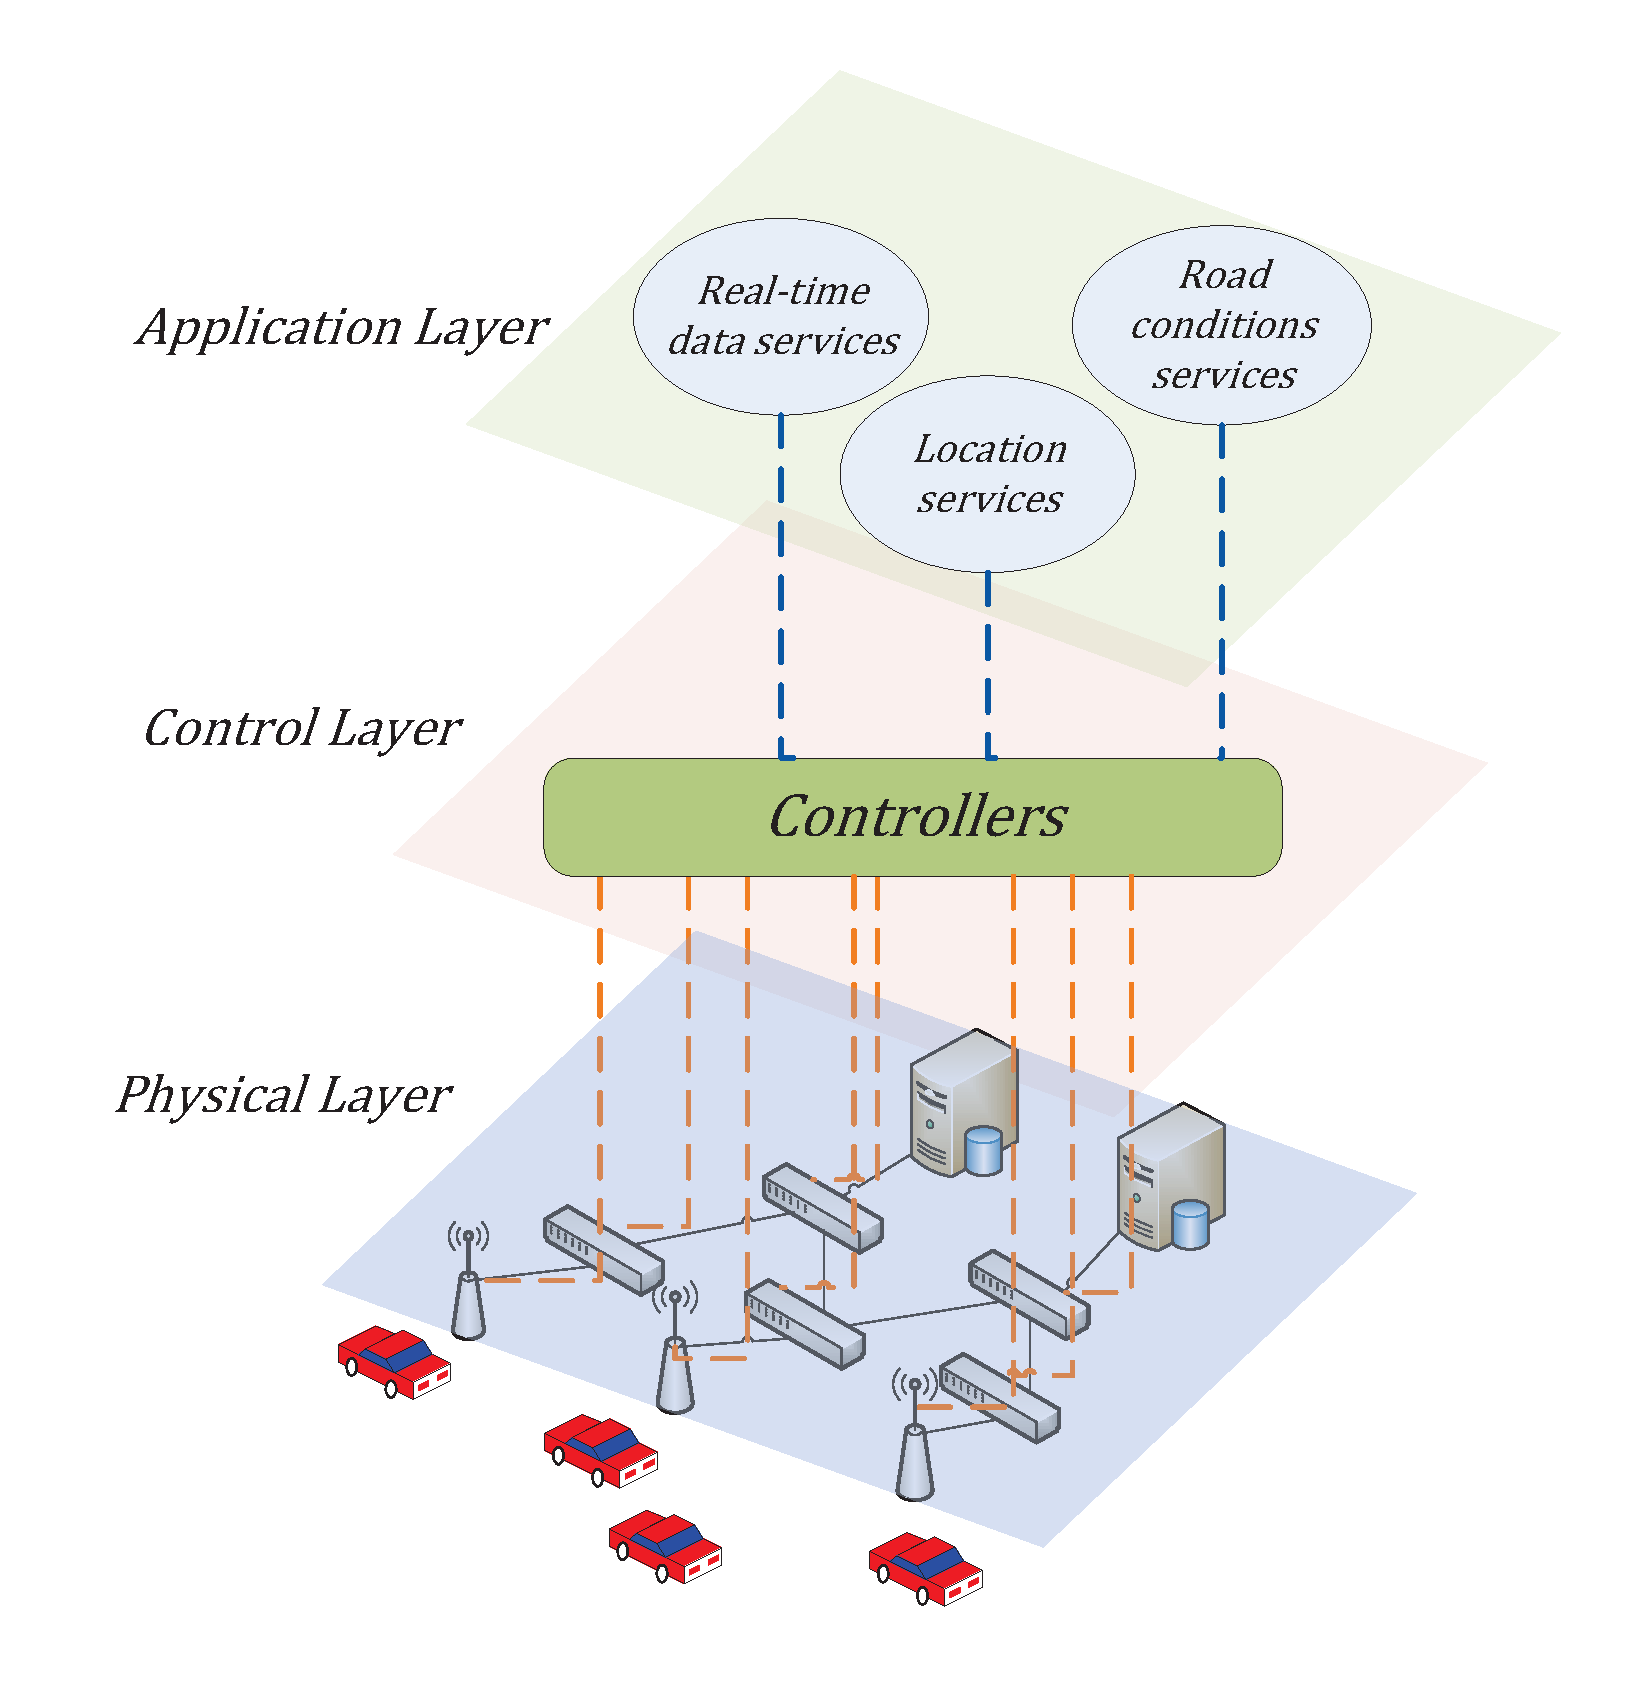
\includegraphics[width=0.9\columnwidth,height=2.5in]{fig-2-24.eps}
\vspace{-0.2in}
\caption{Three-tier SDIV architecture with physical layer, control layer and application layer from bottom to top.} \label{fig2}
\end{center}
\vspace{-0.3in}
\end{figure}

After introducing the SDIV components, we describe how SDIV works with two scenarios as depicted in Fig. ~\ref{fig3}.


\begin{figure} [t]
\begin{center}
\begin{tabular}{c}
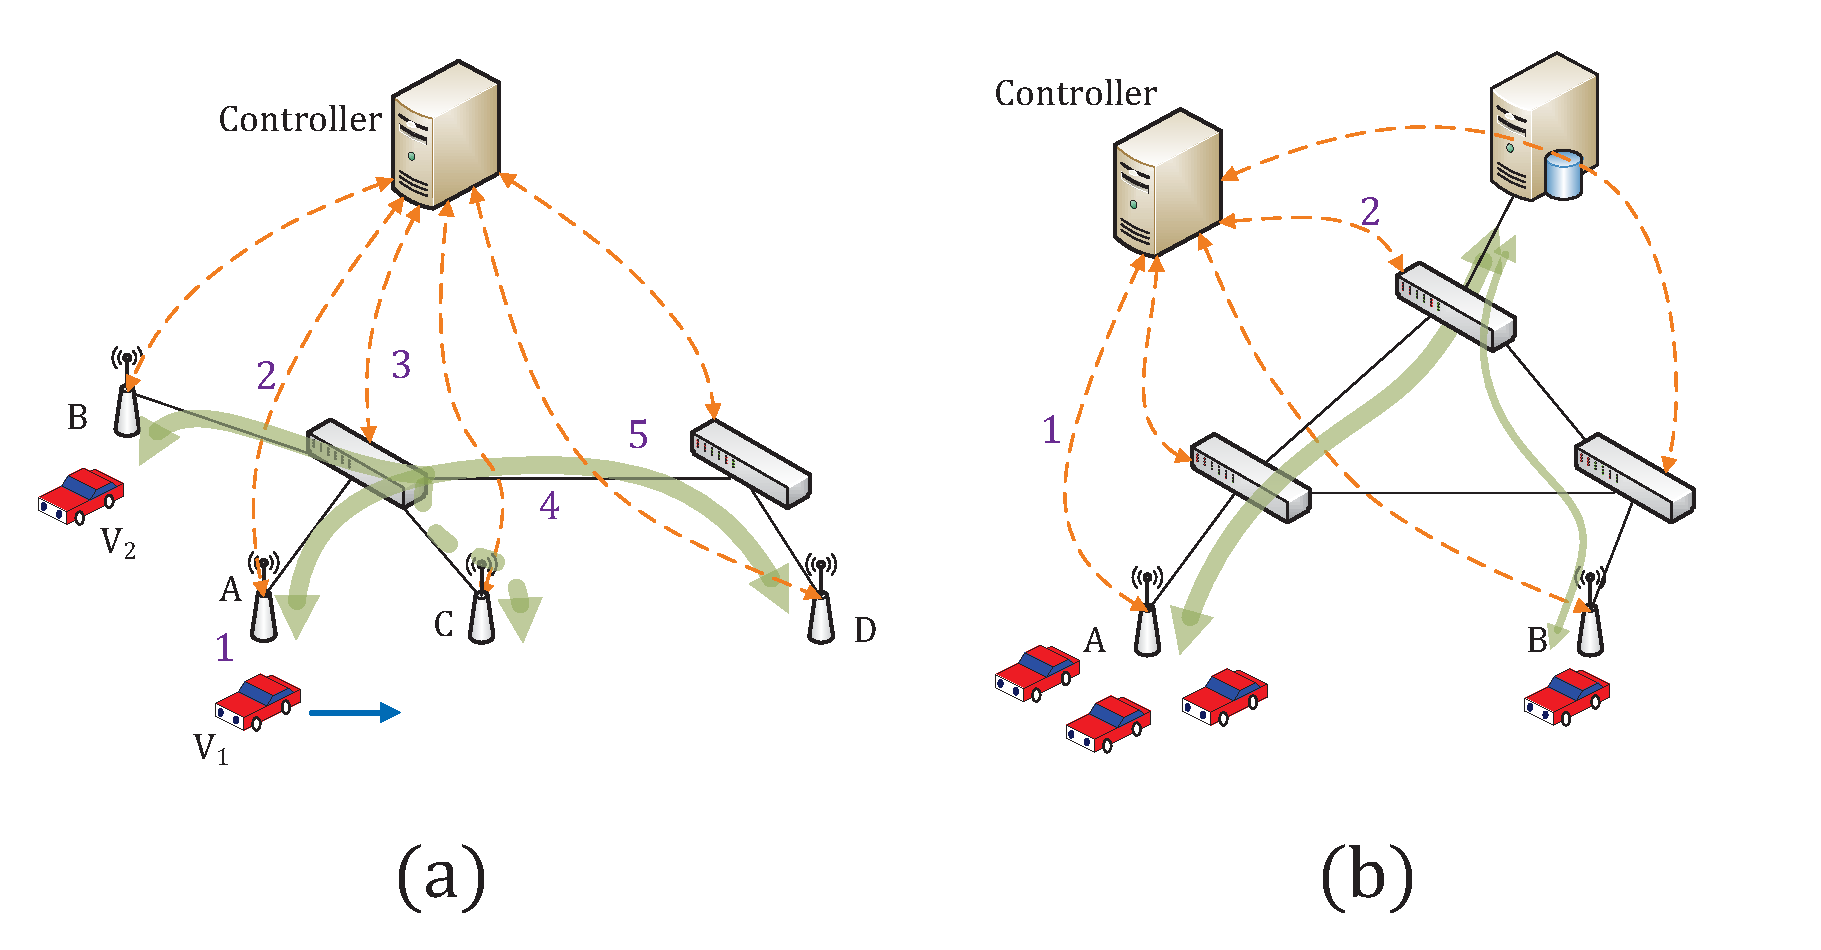
\includegraphics[width=1\columnwidth]{fig-3-29.eps} \\
\end{tabular}
\caption{\textcolor{blue}{(a): A scenario shows, by analyzing vehicle conditions, the controller can install rules (dash line) in advance to avoid extra queries; (b): A scenario of achieving intelligent bandwidth allocation based on a global view in the controller.}} \label{fig3}
  \end{center}
  \vspace{-0.3in}
\end{figure}

Fig. ~\ref{fig3}(a) describes a typical scenario where a vehicle wants to receive the information about road conditions (maybe three blocks away from its current location) via surveillance cameras.

In Step 1, vehicle $V_{1}$ sends a request to a nearby road-side AP as shown in Fig.~\ref{fig3}(a); in Step 2, since there is no rule matching the header of the flow's first packet, the switch (AP $A$) encapsulates and forwards the packet to the controller; in Step 3, the controller recognizes the header and installs rules based on the vehicle's requests and information (e.g., location, speed and direction) and also the current network state; in Step 4, switches along the path towards the destination forward the matched packet to given ports based on the rules installed; in Step 5, the data flow from the surveillance camera ($D$) to the vehicle, goes through the same procedure as described in Steps 2-4. When the number of vehicles increases ($V_{2}$ at $B$ appears), there needs a scalable approach to installing rules for data transmission. The conditions (e.g., directions) of vehicles should be considered for installing rules, e.g., installing rules at $C$ in advance.

Fig.~\ref{fig3}(b) describes a scenario where vehicles need to build connections with the server through nearby APs for data uploading such as their current speed and location. The upper layer application (different from the servers in the network) can benefit from the data uploading scenario for analyzing road conditions. If the controller receives many packets from a particular AP, it can tell that there are many vehicles in this area compared with other places receiving few packets only. In Step 1, the controller gathers the information from APs $A$ and $B$. When switches receive packets with no rule matching, they send the packets to the controller. In Step 2, the controller installs rules in switches according to the destination addresses. If the upper layer application finds more vehicles in $A$ than in $B$, it can allocate more bandwidth to $A$.

In addition, SDIV is more attractive when considering large-scale multicast and mobility of vehicles. As the number of vehicles connecting to one camera increases, it is easy to think of multicast for the efficiency of data transmission. Although dense-mode multicast (reasonable for cameras) goes well in small networks, as the range of data transmission increases, the growing number of $(S,G)$ \textcolor{blue}{(S: Source IP, G: Group IP)} entries kept in APs (or switches) and broadcasting messages periodically for establishing shortest path tree (SPT) limit the scalability of data transmission. The mixed model of control and data planes makes it necessary to keep $(S,G)$ entries even not used currently at every router for a fast graft. In Fig.~\ref{fig3}(a), it is necessary to reserve $(S,G)$ entries at AP $B$ for a new coming vehicle $V_{2}$. The mobility of vehicles also brings difficulty to traditional network technologies. Vehicle $V_{1}$ moving from $A$ to $C$ as described in Fig.~\ref{fig3}(a) needs to send another request for retrieving data, which results in interruption of data stream and extra workload of the surveillance camera ($D$). In our design, we address the mobility problem by predicting the most possible path that the vehicles would choose and set the rules in flow tables in advance to multicast the packets from nearby APs along the path. Multicast along the data transfer path in SPT cannot address the mobility issue since the shortest path for data transmission seldom matches the driving path.

Table 1 summarizes the benefits of SDIV against traditional network technologies (multicast) besides its open interface of network equipment. Compared to the traditional multicast method that needs to broadcast messages periodically for establishing SPT, SDIV leverages the benefits of OpenFlow that makes switches forward packets with no matching rule in a flow table to the controller and then the controller installs rules for the packets. It is a reactive mode and rids the need to broadcast messages periodically. This reactive mode also makes it possible that the switches only need to keep the least number of rules in their flow tables instead of keeping $(S,G)$ entries at routers in a traditional multicast method. With the support of an up-to-date, global view of the network topology and traffic states, the application in the controller is able to compute the most possible path that a vehicle would choose and installs rules in advance for providing persistent connection between vehicles and devices.

\begin{table}[t]
 \caption{\label{table1}Pros and cons of traditional network technologies (multicast) and SDIV}
 \centering
 \begin{tabular}{c|c}
  \hline
  Traditional Technologies & SDIV \\
  \hline
  \hline
 \Gape[4pt] Con: Broadcasting messages periodically & Pro: Reactive mode \\
 \hline
 \Gape[4pt]Con: Keeping $(S,G)$ entries at routers& Pro: Installing rules when needed \\
 \hline
 \Gape[4pt]Con: SPT cannot match the driving path & \tabincell{c}{Pro: Finding the path according to \\the direction of vehicles}\\
  \hline
  \Gape[4pt]Pro: Do not need a controller & Con: Need a controller \\
  \hline
 \end{tabular}
 \vspace{-0.295in}
\end{table}


\section{Improved Rule Installation} \label{Rule Optimization}

Having described the SDIV architecture and how SDIV works, we give a solution for the rule installation problem and explain that it could bring significant complexity and overhead if naively installing rules are adopted for packet forwarding. We consider a real-time query service as the context to explain the necessity of its optimal solution.

In a real-time query service, if the controller simply installs rules for the requests from drivers, the size of flow tables will incur the performance bottleneck due to the limited size of ternary content-addressable memory (TCAM) in switches. Thus, it is important to produce compact tables to fit more cached policy decisions in the switches. For each flow established, two rules are needed at the selected switches for sending the request packets and receiving the packets from the destination. Even if we only consider the second data flow, since the request flow is only useful at the beginning and can be deleted via timeout mechanism in OpenFlow switches, we still need at least one rule for each flow. It sounds that one rule for each flow is compact enough for a flow table, but in reality drivers attempt to connect multiple surveillance cameras at the same time. As a result, we need to install rules for every such data flow at every selected switch even though these flows all have the same destination. To summarize, we have to reduce the number of packets forwarded to the controller and establish a compact flow table due to the limited size of TCAM at switches.

Fig.~\ref{fig4} depicts the basic scenario that how a real-time query service works. Suppose that $V_{1}$ wants to obtain the conditions of road (or crossroads) $E$. Here, the conditions can be a video or any other kinds of data stored in the roadside devices. At the first step, $V_{1}$ sends a request to AP $A$ and then the data flow is forwarded to $E$. After confirming the request from $V_{1}$, $E$ sends data to AP $A$. Finally, AP $A$ transmits the data to $V_{1}$ and completes the data transmission. The entire process is simple, but the simplicity may introduce significant performance penalty. As shown in Fig. ~\ref{fig4}, consider the situation that there is another vehicle $V_{2}$ that wants to get the information of $E$. And also the $V_{2}$ is ahead of $V_{1}$. When $V_{2}$ follows the same procedure as $V_{1}$ does, there is another path from $E$ to $B$ established, which makes switch $D$ install two rules following the same path. As the result, as the number of vehicles connecting to $E$ increases, the flow table size at switches along the path may reach the maximum that in turn reduces the performance of the real-time query service. Moreover, when $V_{1}$ moves to another place, it needs to send a request again.



Next, we consider another example to show the importance of optimal rule installation. $V_{1}$ wants to get the data from $E$ and $F$ at the same time. Switches $B$ and $D$ need to install more rules to make data flow transmitted to $A$, even though both flows ($E \to A$ and $F \to A$) have the same destination. Such situations become more complex if $V_{3}$ requests the same service. To enable $V_{3}$ at $C$ to receive data, there is a need of building a new path (i.e., the same data flow will split at the attaching switch of the three vehicles, then the switch becomes a branching node), which again increases the flow table size. The mobility of vehicles increases the complexity and degrades performance of the real-time query service as well.

To solve the rule installation problem and mitigate the flow table size growth, we propose to separate the wireless data plane (for communication between vehicles and APs) from the wired data plane (for communication among switches) and develop a destination-driven model (given later in Section ~\ref{Modify address}) for the wired data plane. When vehicles receive data from nearby APs, they do not care how data transmitted in the wired data plane. Instead, they just want a persistent connection even their locations change over time. To make the separation efficiently, we introduce three techniques: (1) using a multicast address as the last hop address from cameras to vehicles, (2) installing rules in the most possible path in advance according to the conditions of vehicles, and (3) modifying the headers when packets come to branching nodes to be defined.


%\begin{figure} [t]
%\begin{center}
%\includegraphics[width=0.7\columnwidth]{fig5-modified-type-large.eps}
%
%\caption{A separation between wired data plane and wireless data plane. Dash line means that data flow may be established incrementally from a existing one.} \label{fig5}
%\end{center}
%\end{figure}




\subsection{Multicast Address for the Last Hop} \label{Multicast address}



We utilize multicast addresses for the purpose to deal with the mobility and enhance the scalability of SDIV. Every surveillance camera has a unique multicast address which can be generated from a MAC address by the same method in traditional networks. Multicast addresses can be used in the last hop from cameras to vehicles for data transmission in the wireless data plane. Vehicle $V_{1}$ receives packets with the destination address of $E$'s multicast address in Fig.~\ref{fig4}. The advantage of using multicast addresses is apparent, i.e., every vehicle, within the range of an AP that has been equipped with the rule, can get the real-time data without sending new requests. Furthermore, in a real-time query service, the first packet of user requests has to be forwarded to the controller for installing rules. If every request needs to contact the controller for rule installation, it leads to a serious bottleneck at the controller since both computational capacity and bandwidth are limited. A multicast address can address this problem efficiently. After the first vehicle connected the camera with the intervention of the controller, the data flow starts to multicasts (along the path to the destination), and every new vehicle asking for the same camera receives the data without sending the request, which reduces the frequency of contacting the controller. For example in Fig.~\ref{fig4}, if there is another vehicle that wants to see the conditions of $E$, it can receive the data without sending a request after $V_{1}$ sent the request.

Due to the limited size of TCAM in OpenFlow-supported switches, we need to remove the useless rules from flow tables. In our design, we use timeout in OpenFlow to delete rules for saving flow table resources. A switch maintains a per-flow-entry variable that indicates if there has ever been a period of $T$ seconds in which no packet arrived for the flow. In practice, in OpenFlow, this is maintained by adding an ``idle timeout" value to a flow entry. Instead of setting equal values of timeout, we choose different values of timeout in switches depending on the distance away from the destination. In reality, the number of vehicles interested in the destination gets larger as they are closer to the destination. Then we set larger values in timeout for the closer switches to the destination. As an example in Fig. ~\ref{fig4}, the timeout value $T_{i}$ in switch $i$ meets the constraint: $T_{A} < T_{B} < T_{D} < T_{E}$. The closer to the information source, the less changes on data flows, since these flows would merge to a stable singe flow. The stable data flow would require a long timeout than unstable flows.


\begin{figure} [t]
\begin{center}
\includegraphics[width=1\columnwidth]{fig-4-31.eps}

\caption{$V_{1}$ is connecting to $E$ and $F$ simultaneously, and $V_{2}$ at the path of $V_{1}$ to $E$ asks the data from $E$. $V_{3}$ also requires the data from $E$ but at the different path.} \label{fig4}
\end{center}
%\vspace{-0.3in}
\end{figure}

\subsection{Predicting a Path and Installing Rules in Advance} \label{Predict the path}

\begin{algorithm}[t]
\caption{PathFind($s,d,v$)}
\label{Algorithm 2}
\begin{algorithmic}[1]
%\algsetup{linenosize=\footnotesize}
%\footnotesize

\STATE{Algorithm PathFind($s,d,v$)}
\STATE{~~put $s$ into set $N$, $R$;}
\STATE{~~for each child node $c$ of $s$}
\STATE{~~~~if the angle between $v$ and $A(s,c)$ is less than 90 degree then}
\STATE{~~~~~~put $c$ into set $O$;}
\STATE{~~Find($s,O,d$);}
\STATE{~~return $R$;}
\STATE{Procedure Find($p,O,d$)}
\STATE{~~put $p$ into set $N$;}
\STATE{~~for each $n$ in $O$}
\STATE{~~~~if $n$ is $d$ then}
\STATE{~~~~~~put $n$ into set $R$;}
\STATE{~~~~~~finish;}
\STATE{~~~~put $n$ into set $N$;}
\STATE{~~~~remove $n$ from set $O$;}
\STATE{~~~~calculate $D(n,d)$, $D(p,n)$;}
\STATE{~~~~if $D(p,n)+D(n,d)<max$ then}
\STATE{~~~~~~$max = D(p,n)+D(n,d)$;}
\STATE{~~~~~~$r = n$;}
\STATE{~~put $r$ into set $R$;}
\STATE{~~for each child node $c$ of $r$}
\STATE{~~~~if $c$ not in set $N$ then}
\STATE{~~~~~~put $c$ into set $O$;}
\STATE{~~Find($r,O,d$);}
\STATE{~~return;}
\end{algorithmic}
\vspace{-0.06in}
\end{algorithm}




To deal with the mobility of vehicles in SDIV, it is necessary to predict the most possible path that a driver chooses and then install rules in advance along the path in order to keep data transmission uninterrupted while the vehicle is moving. A simple method to predict such a path is computing the shortest path, but it is not always a correct path in reality. We propose and describe $PathFind(s,d,v)$, in Algorithm 1 that finds the most likely path in a topology. Here $s$ is the current location, $d$ is the destination and $v$ is the direction of the vehicle. $A(s,c)$ denotes the angle of $s$ and $c$, $D(n,d)$ means Euclidean distance between $n$ and $d$. Note that Manhattan distance may also be used to cope with an urban environment.

As the preparatory work (Lines 3-5), $PathFind$ filters the possible first node of a resulting path according to the condition (e.g., direction) of the vehicle, since the driver seldom turns back in a street. We apply $Find$ recursively to calculate the resulting path by choosing the node that has the minimum value of $D(p,n)+D(n,d)$, e.g., the distance between the chosen location and the destination as shown in Lines 17-20. In the current design, $D(n,d)$ denotes Euclidean distance between $n$ and $d$, but we can change it to a more intelligent calculation. Finally, $Find$ identifies the destination as the next node and returns the result (Lines 12-14).

We apply $PathFind$ in Fig.~\ref{fig5}. Consider a vehicle in location $A$ plans to find a path to $F$. First, it puts $B$ into set $O$ according to the direction of the vehicle at the current location. It then finds $D$ has a shorter path to $F$ compared with $C$. It chooses $D$ to start again, and finds $D$ that directly connects to $F$ and finishes. The result $A \to B \to D \to F$ is more reasonable than the shortest path $A \to E \to F$ since reversing a vehicle is rarely seen in reality (unless the distance difference is quite large). Though the delay of path $A \to B \to D \to F$ is prolonged comparing to path $A \to E \to F$, the vehicle sends more requests when it finds no data from its nearby AP. In this case, the vehicle more likely chooses $B$ as its next location, and thus the resulting path is better than the shortest path since the vehicle can receive data without sending another request. In Fig. ~\ref{fig5}, after installing rules at the switches along the predicted path ($A \to B \to D \to E$), the multicast address also makes $V_{2}$ receive data without sending a new request.




\subsection{Modifying Address in Branching Nodes} \label{Modify address}

\begin{algorithm}[t]
\caption{ModifyAddress($s,d,path$)}
\label{Algorithm 3}
\begin{algorithmic}[1]
%\algsetup{linenosize=\footnotesize}
%\footnotesize

\STATE{Algorithm ModifyAddress($s,d,path$)}
\STATE{~~for each node $n$ in $path$ do}
\STATE{~~~~$nx$ = the next node of $n$;}
\STATE{~~~~$setRule$ = false;}
\STATE{~~~~for each rule $r$ in $n$ do}
\STATE{~~~~~~$no$ = the node connecting the output port of $r$;}
\STATE{~~~~~~if $r$ matching $s$ and $no$ != $nx$ then}
\STATE{~~~~~~~~$act$ = forward to $nx$ and modify the destination address to $d$;}
\STATE{~~~~~~~~$emitRule(matchFor(d),act)$;}
\STATE{~~~~~~~~$setRule$ = true;}
\STATE{~~~~~~else if $r$ matching $s$ and $no$ = $nx$ then}
\STATE{~~~~~~~~$setRule$ = true;}
\STATE{~~~~if $setRule$ == false then}
\STATE{~~~~~~$act$ = forward to $nx$;}
\STATE{~~~~~~$emitRule(matchFor(d),act)$;}
\STATE{~~return;}
\end{algorithmic}
\vspace{-0.06in}
\end{algorithm}

\vspace{-0.05in}

\begin{figure} [t]
\begin{center}
\includegraphics[width=0.9\columnwidth]{fig-5-31.eps}

\caption{The blue dash line is the shortest path between current location and destination, while the red dash line is a more likely path that the vehicle may choose according to the direction.} \label{fig5}
\end{center}
\vspace{-0.3in}
\end{figure}

In this subsection, we will show how to install rules at switches. The main idea is that we add a packet header modifying action at the branching nodes (Line 8-9) by leveraging the properties of OpenFlow as shown in Algorithm 2. The input $s$ denotes the source of data, $d$ denotes the current location of the vehicle and $path$ is computed by $PathFind$. \textcolor{blue}{When a packet matches a rule to modify the match field, it will first apply the modification before forwarding to a particular port, and this process is guaranteed by the OpenFlow protocol. The modified address makes the packet forwarded to the switch directly connecting to the vehicle.} We clarify that the rule matching $s$ means that the controller records the source address of every request, not the rule in the switch matches $s$. By using the address modification algorithm, we let packets with different source addresses but the same destination address match the same rule and hence reduce the number of rules and reduce the flow table size. We call this approach a destination-driven model, since it needs to match the destination address only.

As an example shown in Fig.~\ref{fig6}, data flows $F_{1}$ and $F_{2}$ are both generated from surveillance camera $S_{1}$, and $F_{3}$ comes from $S_{2}$. $F_{1}$ is requested from $V_{1}$. $F_{2}$ and $F_{3}$ are destined to $V_{2}$. Suppose that $V_{1}$'s current location is $C$ and $V_{2}$ is at $D$, $F_{1}$ and $F_{2}$ need at least two rules at switches $A$ and $B$ in unicast, and $F_{2}$ and $F_{3}$ need two rules at least at switches $A$ and $B$ in multicast. This is not efficient since $F_{1}$ and $F_{2}$ come from the same node, and $F_{2}$ and $F_{3}$ have the same destination. We modify the destination address in the header of packets in switch $B$ (as a branching node) for $F_{1}$ and $F_{2}$. By setting the destination address of packets in $F_{1}$ and $F_{2}$ ($F_{1} \to C$ and $F_{2} \to D$), the number of rules in switches is reduced and so is the size of the flow table for more services. Let's assume $V_{2}$ sends a request to $S_{1}$ in the beginning. Each switch only needs one rule to carry $F_{2}$. When $V_{2}$ asks data from $S_{2}$, the rules at switches still suit. Finally, when $V_{1}$ requires data from $S_{1}$, it just increases one rule at switch $B$ via matching $(S_{1}, D)$ with an action of modification. Here we use two parameters to represent the packet header, namely $(source address, destination address)$, and so are the match conditions in the flow table. This destination-driven mode emphasizes the destination address as matching conditions in the flow table, and generalizes the data flow demands of the same destination for reducing the size of flow tables in switches. In Fig.~\ref{fig4}, when $V_{3}$ joins, it needs address modification at the branching switch to optimize rule installation.

Next, we give an analysis of improved rule installation for two cases: (a) one server connects to multiple vehicles and (b) one vehicle connects to multiple servers. For the first one, the traditional rule installation that forwards packets to given ports simply based on the source address needs one rule at each switch along the data path. In our proposed rule installation method, we need one rule at each switch for forwarding and an extra action for modifying data header at the branch nodes. Since the modifying address action can be combined with the forwarding action in OpenFlow as a set of actions of rule, the number of rules does not change compared with the traditional rule installation. For the second one, we assume that there is one vehicle ($v$) connecting to multiple servers ($s_1, s_2,...s_n$), and $s_i$ is $h_i$ hops away from $v$. Let $L_i$ denote a set of links used for the data flow between $v$ and $s_i$. Hence, we have $|L_i| = h_i$. Then the traditional approach needs $\sum_{i=1}^{n} h_i$ rules, while by our improved rule installation, we need $|L|$ rules where $L = \bigcup{(L_{1}, L_{2}, ... L_{n})}$. Considering one extreme scenario that any two $L_i$ and $L_j$ have no sharing link. Then we have $|L| = \sum_{i=1}^{n} h_i$. In this scenario, the number of rules needed by the proposed approach is the same as the traditional method. For many other scenarios, $|L| < \sum_{i=1}^{n} h_i$, which means that the use of the proposed one reduces the number of rules. In summary, the worst case of our improved rule installation including the case one and the extreme scenario of case two does not change the number of rules while the best case could reduce many rules when there is one vehicle connecting to multiple servers.




\begin{figure} [t]
\begin{center}
\includegraphics[width=1\columnwidth]{fig-6-31.eps}
\caption{Data flow $F_{1}$ (red line) comes from $S_{1}$ and its destination is $C$; Data flow $F_{2}$ (blue line) comes from $S_{1}$ and its destination is $D$; Data flow $F_{3}$ (green line) comes from $S_{2}$ and its destination is $D$. The matching conditions only depend on the destination address.} \label{fig6}
\end{center}
\vspace{-0.3in}
\end{figure}

\begin{figure*} [t]
\begin{center}
\begin{tabular}{cc}
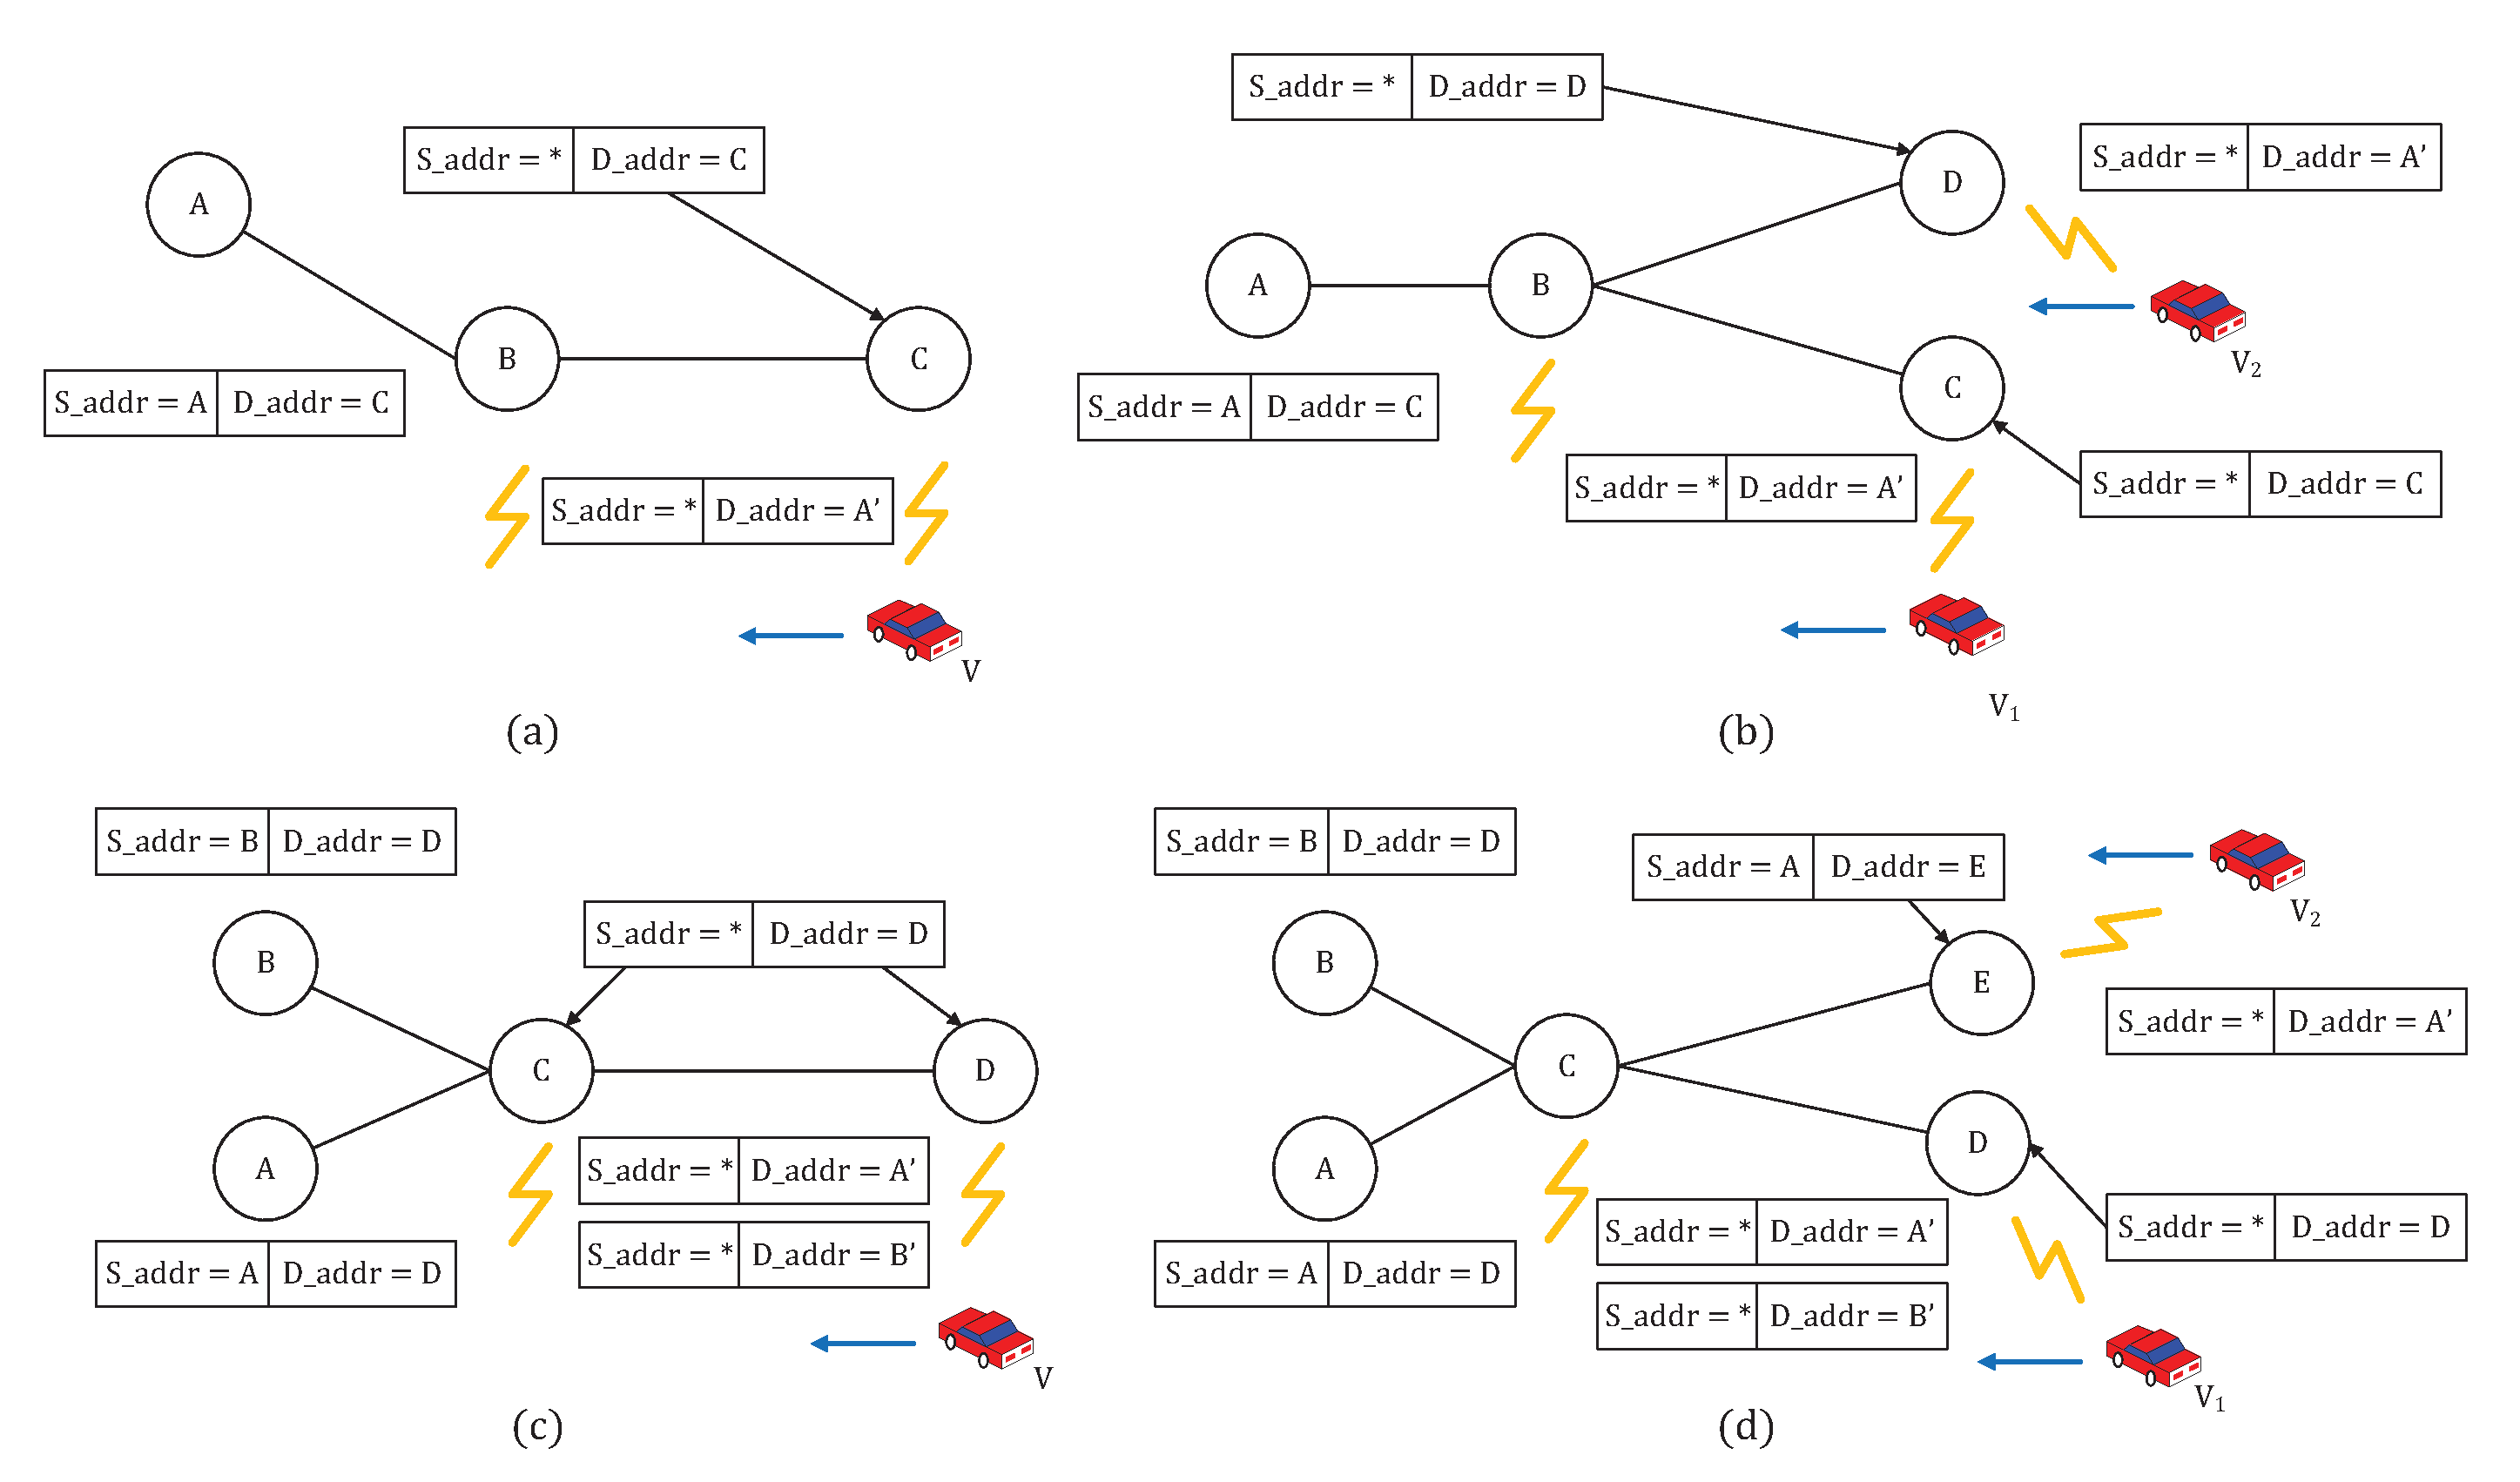
\includegraphics[width=1.9\columnwidth]{fig8-big.eps}
\end{tabular}
\caption{(a): a \textit{one-to-one} pattern that $V$ wants to receive data from $A$; (b): a \textit{N-to-one} pattern that $V_{1}$ and $V_{2}$ want to receive data from $A$; (c): a \textit{one-to-N} pattern that $V$ wants to receive data from $A$ and $B$ at the same time; (d): a \textit{N-to-N} pattern that $V_{1}$ wants to receive data from $A$ and $B$ while $V_{2}$ wants to receive data from $A$.} \label{fig7}
  \end{center}
  \vspace{-0.3in}
\end{figure*}


\subsection{Examples} \label{Examples}



We give four examples to show how our approach works. We then describe the details of rule installation at switches. By analyzing the process of data transmission in a real-time query service, we summarize four patterns as shown in Fig.~\ref{fig7}.

\subsubsection{one-to-one \rm{case}} \label{1 to 1}

In the simplest situation, there is only one vehicle asking for a real-time query service from one surveillance camera. As shown in Fig.~\ref{fig7}(a), $V$ sends a request to camera $A$ and then receives data flow from $A$. The packets from $A$ is $(A, C)$, and matching conditions at $B$ and $C$ are both $(*, C)$. The packets multicast at $C$ is $(*, A^{'})$ where $A^{'}$ is the multicast address of $A$. In this scenario, the path found by $PathFind(s,d,v)$ is $C\to B \to A$, which is the most likely path that the driver would choose. Then we install rules for multicast with $(*,A^{'})$ at $B$ previously. When $V$ arrives at $B$, it can receive data without interruption.


\subsubsection{N-to-one \rm{case}} \label{N to 1}

When a camera connects to multiple vehicles, there is the need to modify the destination address at the branching nodes, e.g., $B$ in Fig.~\ref{fig7}(b). For OpenFlow switches, it supports a set of actions (e.g. packet header modification and forwarding action) at one rule. Hence the modifying action does not need an extra rule. At the beginning, $A$ sends packets $(A, C)$ since $V_{1}$ at $C$ send the request earlier than $V_{2}$ at $D$. When $V_{2}$ sends a request, the controller (not shown in this figure) installs a new rule with a modification action which can be implemented in OpenFlow. As a result, switch $B$ forwards two packets $(A, C)$ and $(A, D)$ to different ports. The data flows forwarded (by AP) at $B$, $C$ and $D$ are all $(*, A^{'})$.



\subsubsection{one-to-N \rm{case}} \label{1 to N}

A vehicle needs to connect to multiple cameras simultaneously. As descried in Fig. ~\ref{fig7}(c), $V$ wants to receive data from $A$ and $B$ at the same time. The packets generated from $A$ and $B$ are $(A, D)$ and $(B, D)$. At switches $C$ and $D$, the matching conditions are both $(*, D)$. There only needs $one$ rule to meet the requirements for different packets. When a packet $(A, D)$ comes to $C$, the rule $(*,D)$ matches it and then forwards to $D$. Switch $D$ follows the same procedure as $C$. $C$ and $D$ also need to change the destination address of their packets for multicast. The packets for multicast at $C$ and $D$ are $(*, A^{'})$ and $(*,B^{'})$, where $A^{'}$ and $B^{'}$ are the multicast address.


\subsubsection{N-to-N \rm{case}} \label{N to N}

We combine the \textit{one-to-N} and \textit{N-to-one} for a more common scenario \textit{N-to-N} in Fig.~\ref{fig7}(d). $V_{1}$ requires real-time data from $A$ and $B$, and $V_{2}$ requires data from $A$ only. There is a modification at $C$ for packets matching $(A, *)$, since $C$ is a branching node when data source $A$ transfers packets to $D$ and $E$ at the same time. The packets from $B$ are forwarded to the given port without modification.

The \textit{N-to-N} scenario is a general case that gives details about how to implement improved rule installation. We observe that the theoretical upper bound of the table size of the proposed improved rule installation approach is related with the number of devices that the driver is connecting to at the same time. $N_{d}$ denotes the number of devices, $R_{0}$ denotes the number of rules for the traditional approach and $R$ denotes the number of rules for the proposed improved rule installation approach. We have $R = R_{0}/N_{d}$ as the upper bound of the table size. In this case, there are all devices connecting to the same switches.

%\subsection{Pearson Social Similarity} \label{Similarity Attraction}
%
%\begin{defn}[Local Activity]\label{Activity}
%
%Let $a_{u,i}^{t}$  denote the local activity
%of node $u$ in a space-crossing community $ComSC_{i}^{t}$ at time $t$. Then,
%$$a_{u,i}^{t}=\frac{\sum_{(u,v) \in ComSC_{i}^{t}} w_{uv}^{t}}{\sum_{(v^{'},v^{''})\in ComSC_{i}^{t}}w_{v^{'}v^{''}}^{t}}, 1\leq i \leq k, v\neq u$$
%where $v^{'}$ and $v^{''}$ are any two nodes in $ComSC_{i}^{t}$; $w_{uv}^{t}$ has been defined in Section \ref{Contact Aggregation}; $k$ represents the number of space-crossing communities; the numerator represents the sum of the encounter ratios between node $u$ and other nodes in community $ComSC_{i}^{t}$ and the denominator represents the sum of the encounter ratios between any two nodes in community $ComSC_{i}^{t}$.
%\end{defn}




\section{Performance Evaluation} \label{Evaluation}

\subsection{Testbed}

We use Floodlight~\cite{Floodlight} as the controller and Mininet~\cite{mininet} to build an SDN environment so as to evaluate the proposed improved rule installation approach in SDIV. We run Floodlight on a server, with 16 AMD Opteron(tm) processor 6172 and 16GB memory. Our server is installed with Linux kernel version 2.6.32. We run Mininet on a separate server. Servers are connected by a 10Gbps Ethernet network.



\subsection{Effects of Improved Rule Installation}

We use the real data of traveling traces in Shanghai city~\cite{shanghai} as a common scenario to show the benefit of improved rule installation. Fig.~\ref{fig8a}(a) shows a snapshot around People's Square in Shanghai. Traveling traces of vehicles are composed of GPS data at different time. The number of vehicles is limited since we are using the real data in Shanghai city but it is enough to show the effects of the proposed approach. At time $t_{1}$, there are only five vehicles in this area. At $t_{2}$, two more vehicles join. At $t_{3}$, $V_{6}$ appears in the area. The appearing time and disappearing time of vehicles are illustrated in Fig.~\ref{fig8a}(b). Interval time between any two moments is 120 seconds. Since these vehicles cannot appear at the exact time, like $t_{1}$ and $t_{2}$ between which the interval time is 120 seconds, we make the vehicle appear at $t_{i}$ if $|t_{i} - t_{real}| < 30$ where $t_{real}$ is the real appearing time of the vehicle. Although these GPS marks at the same moment may not have exactly the same timestamp, one can say that these vehicles move to these locations very closely at that moment by limiting the difference between the timestamps of GPS marks and the time of moments to a certain range. In this case, we set it to 30 seconds to ensure that every GPS mark can reflect the real location at that moment.

Fig.~\ref{fig8a}(c) is a sketch map of Fig.~\ref{fig8a}(a). Arrows with different features illustrate the directions of vehicles according to the order of these timestamps in GPS marks as shown in Fig.~\ref{fig8a}(a). We assume that there is always one road-side AP (switches in Fig.~\ref{fig8a}(c)) around the GPS marks for data transmission available at any time. We make every vehicle in the sketch map have a data transfer demand at the first moment they appear. Therefore, $V_{1}$ and $V_{2}$ near the intersection of lines 8 and 2 want to receive data from both $B$ and $C$, and also have the same path along line 8. $V_{3}$ locating at the convergence of two roads demands data from $B$ and $C$. $V_{4}$-$V_{5}$-$V_{6}$ have the same target $A$ but choose different paths. $V_{7}$ asks the data from $D$. $V_{8}$ has the target $B$ only. All these vehicles require a persistent data flow service until they move to their destinations. We need to install rules at every necessary switches to meet their requirements.

The baseline method with which we compare is a general method that forwards packets to given ports simply based on the source address. By improved rule installation, we merge the rules that have the same destination (destination-driven mode) in \textit{one-to-N} pattern like $V_{3}$ connecting to $B$ and $C$, and modify headers of packets at branching nodes in \textit{N-to-one} pattern. The result is shown in Fig.~\ref{fig8b}(a). The decline at $t_{4}$ is due to the timeout in rules we set. Fig.~\ref{fig8b}(b) shows the number of vehicles at different moments. Fig.~\ref{fig8b}(c) shows the delay time of different vehicles in two approaches. The delay time we evaluate here is the longest one if a vehicle connects two cameras at the same time. We choose $C$ instead of $B$ for evaluating $V_{1}$'s delay time.

Also, we can observe from Fig.~\ref{fig8b}(c) that our improved rule installation approach hardly affects the performance of data transmission though it needs address modification in the header of packets. We reduce the number of rules and save the space at the flow table for manageability and scalability. Especially, from Fig.~\ref{fig8b}(b), the number of rules has reduced by 60\% comparing with the baseline method.

\begin{figure} [t]
\begin{center}
\begin{tabular}{c}
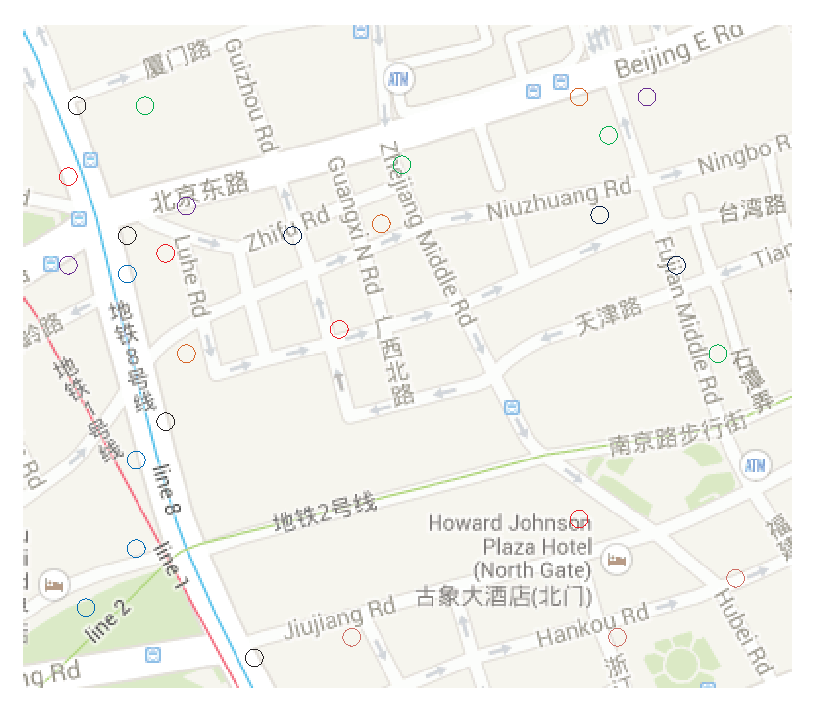
\includegraphics[width=0.85\columnwidth]{fig-e-map-26.eps} \\
(a)
\end{tabular}
\begin{tabular}{cc}
\includegraphics[width=0.45\columnwidth]{fig-e-length-2.eps}&
\hspace {-0.1in}
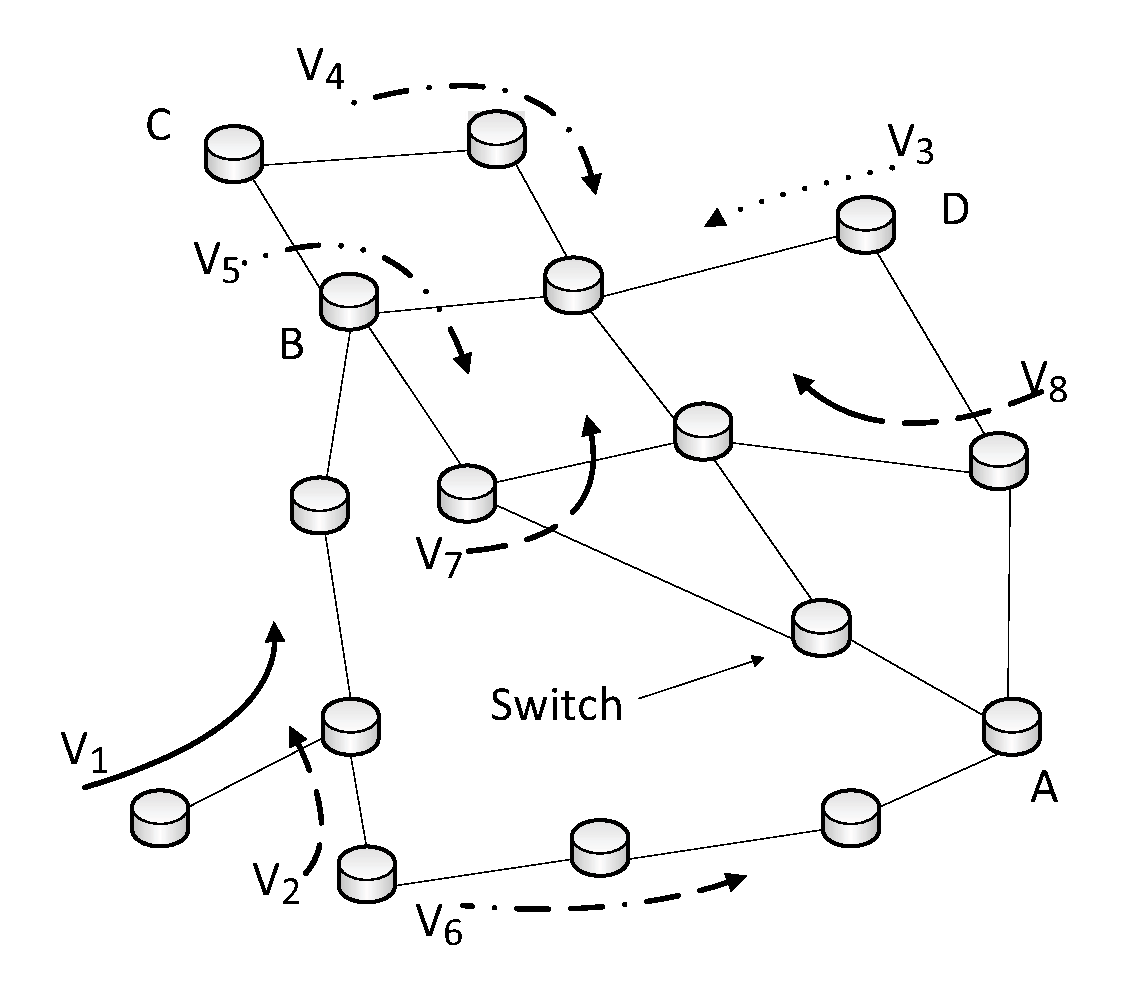
\includegraphics[width=0.45\columnwidth]{fig-e-map-s-26-1.eps} \\
(b) & ~~~(c)
\end{tabular}
\caption{(a): A snapshot around People's Square in Shanghai; (b): The appear and disappear time of vehicles; (c): A sketch map of (a) with the direction of vehicles.} \label{fig8a}
  \end{center}
  \vspace{-0.35in}
\end{figure}

\begin{figure} [t]
\begin{center}
\begin{tabular}{cc}
\includegraphics[width=0.5\columnwidth]{fig-e-num-1.eps}&
\hspace {-0.2in}
\includegraphics[width=0.5\columnwidth]{fig-e-num-2.eps} \\
(a) & (b)~~~
\end{tabular}
\begin{tabular}{c}
\includegraphics[width=0.9\columnwidth]{fig-e-8bar-30.eps} \\
(c)
\end{tabular}
\caption{(a): Different number of rules for two strategies; (b): The number of vehicles at different moments; (c): The delay time of vehicles in two strategies.} \label{fig8b}
  \end{center}
  \vspace{-0.35in}
\end{figure}

\subsection{Delay Analysis}

We study two patterns (\textit{one-to-N} and \textit{N-to-one}) in details and show how they influence results differently. We compare the number of rules and the delay time with the baseline method to show that it does not affect the performance of data transmission. Fig.~\ref{fig9}(a) shows \textit{N-to-one} mode that there are multiple vehicles connecting to one surveillance camera ($B$). We pick $A$ that has the longest path to evaluate delay time. For the baseline method, it needs to install one rule at each switch with the match of source address. And for proposed approach, every packet transferred from $B$ to $A$ modifies the headers (destination IP address) at each switch and then forwards to the next switch. Fig.~\ref{fig9}(b) shows that, as the number of switches increases, delay time of both methods gets larger but with no statistically significant difference. We conclude that the packet modification process in improved rule installation does not influence performance. Fig.~\ref{fig9}(c) shows the number of rules at switches. The red (right side) line represents the baseline method that node $B$ transfers data flow across the network to every node at the same time. It only needs one rule at each switch with $(*, B^{'})$ ($B^{'}$ is the multicast address). The black (left side) line depicts improved rule installation approach that modifies the destination address at every branching node and then forwards the packets to given ports. It needs only one rule at each switch comparing to the the baseline method that requires multiple rules, the number of which equals to the data sources even they have the same destination. For example, the switches along $V_1$ to $B$ need two rules since $V_1$ also sends a request to $C$.

Fig.~\ref{fig9}(d) shows \textit{one-to-N} patterns where vehicle $V$ connects multiple cameras ($B, C, D$) at the same time. Fig.~\ref{fig9}(e) shows the delay time according to the different number of switches. Without improved rule installation, three rules are needed for each source node at each switch, $(B, *), (C, *), (D, *)$, which is a source-driven mode (forwarding packets based on data source). With improved rule installation, we need one rule only, i.e., $(*, A)$ at each switch and it can still support \textit{N-to-one} pattern. Fig.~\ref{fig9}(f) shows the number of rules of two methods.

We draw two conclusions from the results. First, the modification of packets at branching nodes has no impact on the performance of data transmission. Second, for the best case of improved rule installation (\textit{one-to-N}), the number of reduced rules is proportional to the number of data sources. For the worst case of improved rule installation (\textit{N-to-one}), the number of rules at switches is equal to that of the baseline method.

%\begin{figure} [t]
%\begin{tabular}{cc}
%\includegraphics[width=0.5\columnwidth]{fig-e-1-30-a.eps}&\hspace{-0.05\columnwidth}
%\includegraphics[width=0.5\columnwidth]{fig-e-1-30-b.eps}\\
%(a) & (b)
%\end{tabular}
%\begin{tabular}{cc}
%\includegraphics[width=0.5\columnwidth]{fig-e-1-24.eps}&\hspace{-0.05\columnwidth}
%\includegraphics[width=0.5\columnwidth]{fig-e-3-24.eps} \\
%(c) & (d)
%\end{tabular}
%\begin{tabular}{cc}
%\includegraphics[width=0.5\columnwidth]{fig-e-2-24.eps}&\hspace{-0.05\columnwidth}
%\includegraphics[width=0.5\columnwidth]{fig-e-4-24.eps} \\
%(e) & (f)
%\end{tabular}
%\caption{Subfigure (a) shows a topology of \textit{N to 1} mode; (b) shows a topology of \textit{1 to N} mode; (c) shows delay time at different number of switches in (a); (d) shows delay time at different number of switches in (b); (e) shows number rules at different number of switches in (a); (f) shows number rules at different number of switches in (b)} \label{fig9}
%\end{figure}
\begin{figure*} [t]
\begin{center}
\scalebox{0.9}
{
\begin{tabular}{ccc}
\includegraphics[width=0.65\columnwidth]{fig-e-31-a.eps}&
\includegraphics[width=0.65\columnwidth]{fig-e-1-24.eps}&\hspace{-0.1\columnwidth}
\includegraphics[width=0.65\columnwidth]{fig-e-2-24.eps} \\
(a) & (b) & (c)
\\
\includegraphics[width=0.65\columnwidth]{fig-e-31-d.eps}&
\includegraphics[width=0.65\columnwidth]{fig-e-3-24.eps}&\hspace{-0.1\columnwidth}
\includegraphics[width=0.65\columnwidth]{fig-e-4-24.eps} \\
(d) & (e) & (f)
\end{tabular}
}
\caption{(a): A topology of \textit{N-to-one} mode; (b): Delay time on different number of switches in (a); (c): Number rules on different number of switches in (a); (d): A topology of \textit{one-to-N} mode; (e): Delay time on different number of switches in (d); (f): Number rules on different number of switches in (d)} \label{fig9}
  \end{center}
\vspace{-0.3in}
\end{figure*}


\section{Conclusion and Future Work} \label{Conclusion}
This paper proposes a new architecture SDIV to address the proprietary and closed way issue in the traditional network design in IoV. The baseline method of rule installation is not efficient due to the characteristics of IoV. Improved rule installation for reducing flow table size is thus necessary in SDIV. We design an improved rule installation approach that reduces the size of a flow table without degrading the performance of data transmission for real-time query services. The separation of a wired data plane from wireless data plane and the proposed destination-driven mode are suited well for the characteristics of IoV. Evaluation based on testbed implementation with real traces shows that our improved rule installation approach significantly reduces the number of rules without degrading the performance of data transmission. In our future work, we plan to make the controller collect more information from switches, e.g., the counter in the OpenFlow rule which equals the number of matched packets for the rule, for further data transfer optimization.









\bibliographystyle{IEEEtran}
\bibliography{bibsdiv}

\begin{IEEEbiography}[{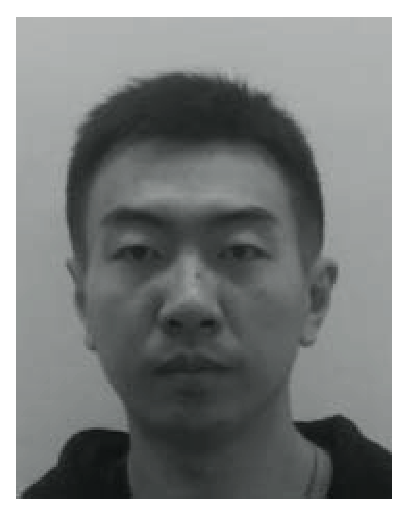
\includegraphics[width=1in,height=1.25in,clip,keepaspectratio]{biophoto/xwang.eps}}]{Xin Wang}
received the BS degree from the Department of Computer Science, Tongji University in Shanghai, China. He is currently working toward the PhD degree in the Department of Computer Science and Engineering, Tongji University. His research interests include computer network, Software Defined Network, and distributed computing.
\end{IEEEbiography}

\begin{IEEEbiography}[{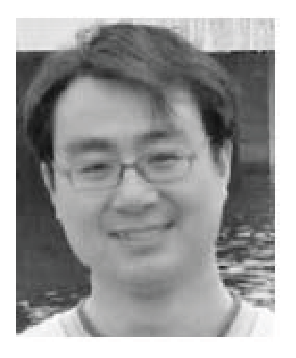
\includegraphics[width=1in,height=1.25in,clip,keepaspectratio]{biophoto/cwang.eps}}]{Cheng Wang}
received MS degree at Department of Applied Mathematics from Tongji University in 2006 and the PhD degree in Department of Computer Science at Tongji University in 2011. He is currently a research professor in the Department of Computer Science at Tongji University. His research interests include software-defined networking, wireless communications and networking, and intelligent transportation system.
\end{IEEEbiography}




\begin{IEEEbiography}
[{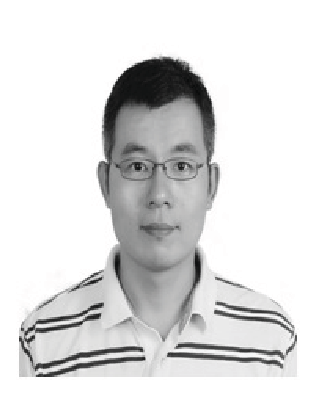
\includegraphics[height=1.35in,clip,keepaspectratio]{biophoto/zhang2014.eps}}]
{Junqi Zhang} received his Ph.D. in Computing Science from Fudan
University, China, in 2007. He became a Post-Doctoral Research Fellow and a Lecturer at the Key
Laboratory of Machine Perception,
Ministry of Education in Computer Science at Peking
university, Beijing, China in 2007, and was the recipient of the Outstanding Post-Doctoral Award
from Peking university. He is currently a Research Fellow and an
Associate Professor with Department of Computer Science and
Technology, Tongji University, Shanghai, China. His current research
interests include machine learning, intelligent and learning
automata, particle swarm optimization,
high-dimensional index and multimedia data
management.
\end{IEEEbiography}



\begin{IEEEbiography}[{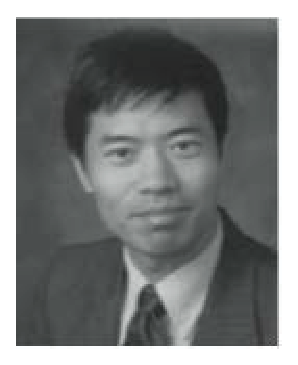
\includegraphics[width=1in,height=1.25in,clip,keepaspectratio]{biophoto/mczhou.eps}}]{Mengchu Zhou}
(S'88-M'90-SM'93-F'03) received his B.S. degree in Control Engineering from Nanjing University of Science and Technology, Nanjing, China in 1983, M.S. degree in Automatic Control from Beijing Institute of Technology, Beijing, China in 1986, and Ph. D. degree in Computer and Systems Engineering from Rensselaer Polytechnic Institute, Troy, NY in 1990.  He joined New Jersey Institute of Technology (NJIT), Newark, NJ in 1990, and is now a Distinguished Professor of Electrical and Computer Engineering. His research interests are in Petri nets, Internet of Things, big data, web services, manufacturing, transportation, and energy systems.  He has over 620 publications including 12 books, 300+ journal papers (240+ in IEEE Transactions), and 28 book-chapters. He is the founding Editor of IEEE Press Book Series on Systems Science and Engineering. He is a recipient of Humboldt Research Award for US Senior Scientists, Franklin V. Taylor Memorial Award and the Norbert Wiener Award from IEEE Systems, Man and Cybernetics Society. He is a life member of Chinese Association for Science and Technology-USA and served as its President in 1999. He is a Fellow of International Federation of Automatic Control (IFAC) and American Association for the Advancement of Science (AAAS).
\end{IEEEbiography}





\begin{IEEEbiography}[{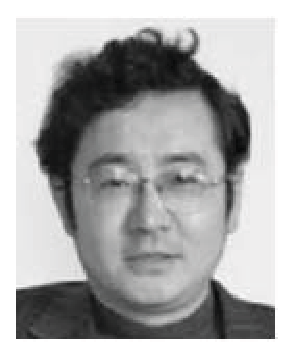
\includegraphics[width=1in,height=1.25in,clip,keepaspectratio]{biophoto/cjjiang.eps}}]{Changjun Jiang}
received the PhD degree from the Institute of Automation, Chinese Academy of Sciences, Beijing, China, in 1995 and conducted postdoctoral research at the Institute of Computing Technology, Chinese Academy of Sciences, in 1997. Currently he is a professor with the Department of Computer Science and Engineering, Tongji University, Shanghai. He is also a council member of China Automation Federation and Artificial Intelligence Federation, the vice director of Professional Committee of Petri Net of China Computer Federation, the vice director of Professional Committee of Management
Systems of China Automation Federation, and an Information Area Specialist of Shanghai Municipal Government. His current areas of research are concurrent theory, Petri net, and formal verification of software, concurrency processing, and intelligent transportation systems. He is a member of the IEEE.
\end{IEEEbiography}
\end{document}


